\chapter{Introduction}

	Following a car crash at the Ketelbrug, we started a design of a safety controller for bridges.
	Several safety concerns are in play, such as the one causing the previously mentioned accident, where the barriers were not closed before the bridge was opened.
	This was caused by an inexperienced operator using the emergency controls,
	which had become commonplace in the operation of that bridge due to problems with the standard controls~\cite{ProjectGuide}.
	
	The design of the bridge's safety controller will have to keep in mind both usability as well as safety.
	The safety of the traffic is the main focus of our safety controller,
	which will check if necessary precautions have been taken to prevent accidents.
	An example would be turning on stop lights before closing the barriers, allowing drivers to slow down in time.
	
	The bridge contains the following components: Pre-signs, Stop-signs, Barriers, Locking pins, Sensors, Brakes, and Motor.
	The safety controller will check the sensors of these components when operating the bridge, and when receiving user command, it will make appropriate decisions to guarantee safety. 
	In \cref{fig:situation} a situation sketch is shown of the system. 
	We assume that the pre-signs are placed a few hundred meters away from the bridge to give drivers an early warning that the bridge is not closed.
	
	\begin{figure}[!htbp]
		\begin{center}
		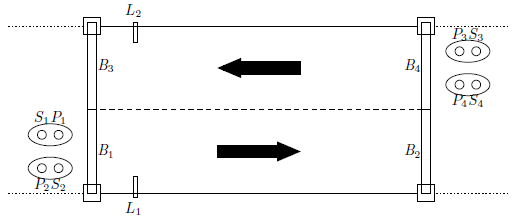
\includegraphics[width=0.6\textwidth]{images/Situation.png}
		\caption{The situation sketch of the system. ~\cite{ProjectGuide}}
		\label{fig:situation}
		\end{center}
	\end{figure}
	
	
	We will now provide the organization of this report. 
	In \cref{chap:requirements} the requirements for the safety controller will be discussed. 
	We will present the architecture of the safety controller in \cref{chap:systemarchitecture}. 
	In \cref{chap:interactions} the interactions between the controller and the other components of the system are described. 
	\cref{chap:tests} presents the transformation of the requirements presented earlier into more specific requirements containing the interactions. 
	This was done using mCRL2. 
	\cref{chap:model} provides information about the model design and all its components. 
	\cref{chap:verification} gives the verification results testing the model with the requirements.
	\cref{chap: conclusion} concludes this report.
